\section{Mapping identifiers to locators in mobile centric architecture}

In order to gain more insights into the requirements of the envisioned mapping scheme and highlight the difference in its usage compared to similar schemes for the LISP proposal, we provide a brief overview of the MobilityFirst architecture, enabling which is a key focus of the XYZ scheme. 

MobilityFirst is a `clean-slate' future Internet architecture project funded by the NSF FIA program~\cite{fia} with a particular focus on supporting large-scale, efficient and robust mobility services in the future Internet. The architecture is motivated by the dramatic growth of mobile devices and applications on the Internet and targets the projected dominance of mobile Internet traffic over that of fixed hosts in the near future~\cite{cisco-2010}. As depicted in Figure~\ref{fig:mobilityFirst} (reproduced from~\cite{nelson-11}), a central principle of the architecture is that every host has a permanent, location independent, globally unique identifier (GUID) which can then be mapped to a set of routable locators or network addresses (NA) corresponding to the current point(s) of attachment. In addition to hosts, GUIDs can refer to content and context to provide seamless content and context handling support in the future Internet. In terms of mapping scheme requirements, this leads to a much larger number of identifiers than the projected number of hosts usually considered in LISP based schemes. The MobilityFirst proposal includes late or repeated binding support, i.e., resolving a GUID to a network address at different points along the route in order to support rapid host mobility. This creates stricter latency requirements for the mapping lookups. Another aspect of the design which affects the mapping scheme is storage aware routing which gives routers the option to temporarily store data as a network-layer routing decision. Retransmitting the stored packets would require another mapping lookup leading to a much higher number of lookups compared to LISP based schemes.

    \begin{center}
        %\vspace{-0.2in}
        \begin{figure}[t]
            \centering
            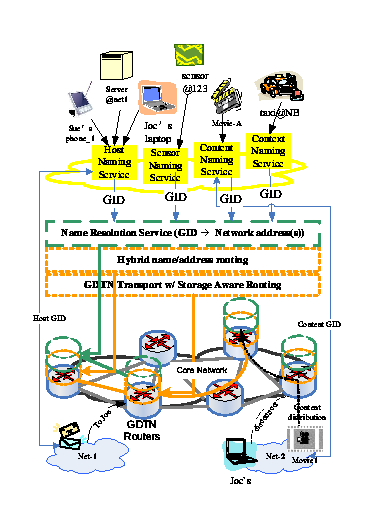
\includegraphics[width=0.8\textwidth]{figures/mobilityFirst.eps}
            \caption{Separation of identifiers (GUID) and locators (NA) in the MobilityFirst architecture}
            \label{fig:mobilityFirst}
        \end{figure}
    %\vspace{-0.2in}
    \end{center}
